\documentclass{standalone}
\usepackage{tikz}
\usepackage{ctex,siunitx,mhchem}
\setCJKmainfont{Noto Serif CJK SC}
\usepackage{tkz-euclide}
\usepackage{amsmath}
\usetikzlibrary{patterns, calc}
\usetikzlibrary {decorations.pathmorphing, decorations.pathreplacing, decorations.shapes,}
\begin{document}
\small
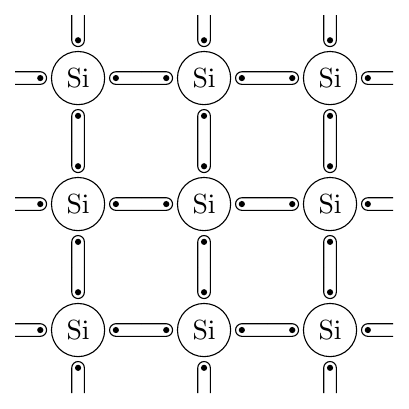
\begin{tikzpicture}[>=latex,scale=1.6]
  \useasboundingbox(-1.4,-1.4)rectangle(1.4,1.4);
  \foreach \x in {-1,0,1}
  {
    \foreach \y in {-1,0,1}
    {
      \node[circle,draw,inner sep=3pt]at (\x,\y){\ce{Si}};
      \fill (\x+0.3,\y) circle (0.7pt);
      \draw (\x+0.5,\y+0.05)--++(-0.2,0)arc(90:270:0.05)--++(0.2,0);
      \fill (\x-0.3,\y) circle (0.7pt);
      \draw (\x-0.5,\y+0.05)--++(0.2,0)arc(90:-90:0.05)--++(-0.2,0);
      \fill (\x,\y+0.3) circle (0.7pt);
      \draw (\x+0.05,\y+0.5)--++(0,-0.2)arc(0:-180:0.05)--++(0,0.2);
      \fill (\x,\y-0.3) circle (0.7pt);
      \draw (\x+0.05,\y-0.5)--++(0,0.2)arc(0:180:0.05)--++(0,-0.2);
    }
  }
\end{tikzpicture}
\end{document}